\documentclass[12pt,a4paper]{book}
\newcommand{\niveau}{5\textsuperscript{e}}
% ================================
% PRÉAMBULE COMMUN — Mathématiques (6e, 5e, 4e)
% ================================

% Encodage et langue
\usepackage[T1]{fontenc}
\usepackage[french]{babel}

% Typographie moderne
\usepackage{newtxtext,newtxmath}

% Configuration des pages
\usepackage{geometry}
\geometry{top=2.5cm, bottom=2.5cm, left=2.5cm, right=2.5cm}

% Amélioration du rendu
\usepackage{microtype}

% Personnalisation des titres
\usepackage{titlesec}
\titleformat{\chapter}[hang]{\huge\bfseries}{\thechapter.}{0.6em}{}
\titleformat{\section}[hang]{\Large\bfseries}{\thesection}{0.6em}{}
\titleformat{\subsection}[hang]{\large\bfseries}{\thesubsection}{0.6em}{}

% Ajustement de l'espacement des titres
\titlespacing{\chapter}{0pt}{-10pt}{20pt}
\titlespacing{\section}{0pt}{12pt}{8pt}
\titlespacing{\subsection}{0pt}{4pt}{2pt}

% En-têtes et pieds de page
\usepackage{fancyhdr}

% Packages mathématiques
\usepackage{amsmath, mathtools}
\usepackage{siunitx}

% Graphiques
\usepackage{tikz}
\usetikzlibrary{angles, quotes, calc, arrows.meta, shapes.geometric}
\usepackage{pgfplots}
\pgfplotsset{compat=1.18}

% Liens hypertexte
\usepackage{hyperref}
\hypersetup{
    colorlinks=true,
    linkcolor=blue!60!black,
    urlcolor=blue!60!black,
    citecolor=blue!60!black
}

% Boîtes colorées avec tcolorbox
\usepackage[most]{tcolorbox}

% Configuration globale des boîtes
\tcbset{
    rounded corners,
    boxsep=2ex,
    top=1.5ex,
    bottom=1.5ex,
    left=2.5ex,
    right=7ex,
    before skip=0pt,
    after skip=1.5ex,
    width=\textwidth,
    boxrule=1pt
}



% Définition des environnements personnalisés
\newtcolorbox{definitionbox}[1][]{
    colback=orange!5!white,
    colframe=orange!70!black,
    title={\textbf{Définition \thechapter.\number\numexpr\thedefinition+1\relax}\ifthenelse{\equal{#1}{}}{}{ : #1}},
    fonttitle=\bfseries,
    coltitle=black,
    before upper={\incdefinition}
}

\newtcolorbox{examplebox}{
    colback=green!5!white,
    colframe=green!60!black,
    title={\textbf{Exemple}},
    fonttitle=\bfseries,
    coltitle=black
}

\newtcolorbox{exercisebox}{
    colback=purple!5!white,
    colframe=purple!70!black,
    title={\textbf{Exercices}},
    fonttitle=\bfseries,
    coltitle=black
}

\newtcolorbox{objectifsbox}{
    colback=teal!5!white,
    colframe=teal!70!black,
    title={\textbf{Objectifs}},
    fonttitle=\bfseries,
    coltitle=black
}

\newtcolorbox{proprietebox}[1][]{
    colback=red!5!white,
    colframe=red!70!black,
    title={\textbf{Propriété \thechapter.\number\numexpr\thepropriete+1\relax}\ifthenelse{\equal{#1}{}}{}{ : #1}},
    fonttitle=\bfseries,
    coltitle=black,
    before upper={\incpropriete}
}

\newtcolorbox{activitybox}{
    colback=blue!5!white,
    colframe=blue!70!black,
    title={\textbf{Activité}},
    fonttitle=\bfseries,
    coltitle=black
}

\newtcolorbox{remarkbox}[1][]{
    colback=yellow!5!white,
    colframe=yellow!70!black,
    title={\textbf{Remarque \thechapter.\number\numexpr\theremarque+1\relax}\ifthenelse{\equal{#1}{}}{}{ : #1}},
    fonttitle=\bfseries,
    coltitle=black,
    before upper={\incremarque}
}

\newtcolorbox{quizbox}{
    colback=cyan!5!white,
    colframe=cyan!70!black,
    title={\textbf{Quiz}},
    fonttitle=\bfseries,
    coltitle=black
}

\newtcolorbox{methodebox}[1][]{
    colback=purple!5!white,
    colframe=purple!70!black,
    title={\textbf{Méthode \thechapter.\number\numexpr\themethode+1\relax}\ifthenelse{\equal{#1}{}}{}{ : #1}},
    fonttitle=\bfseries,
    coltitle=black,
    before upper={\incmethode}
}

% Compteurs pour les environnements (par chapitre)
\newcounter{definition}
\newcounter{propriete}
\newcounter{methode}
\newcounter{remarque}

% Réinitialisation des compteurs au début de chaque chapitre
\makeatletter
\@addtoreset{definition}{chapter}
\@addtoreset{propriete}{chapter}
\@addtoreset{methode}{chapter}
\@addtoreset{remarque}{chapter}
\makeatother

% Commandes pour incrémenter automatiquement les compteurs
\newcommand{\incdefinition}{\stepcounter{definition}}
\newcommand{\incpropriete}{\stepcounter{propriete}}
\newcommand{\incmethode}{\stepcounter{methode}}
\newcommand{\incremarque}{\stepcounter{remarque}}

% Commande personnalisée pour les trous
\newcommand{\trous}[1]{\makebox[#1]{\rule{0pt}{1.2ex}\dotfill}}

% Variable pour stocker le titre de la séquence
\newcommand{\seqtitle}{}
\newcommand{\setseqtitle}[1]{\renewcommand{\seqtitle}{#1}}

% Mise en page de l'en-tête et du pied
\pagestyle{fancy}
\setlength{\headheight}{16pt} % FIX: évite le warning fancyhdr
\fancyhf{}
\lhead{Mathématiques \niveau{} -- 2025--2026}
\rhead{Seq.~\thechapter~--~\seqtitle}
\cfoot{\thepage}

% Listes compactes
\usepackage{enumitem}
\setlist[itemize]{left=1.2em}
\setlist[enumerate]{left=1.5em}

% Configuration des labels personnalisés pour enumitem
\SetEnumitemKey{a}{label=\alph*)}
\SetEnumitemKey{1}{label=\arabic*)}

% Définition des styles de listes personnalisés
\newlist{exerciselist}{enumerate}{1}
\setlist[exerciselist]{label=\alph*)}

\newlist{quizlist}{enumerate}{1}
\setlist[quizlist]{label=\arabic*)}

% Packages pour tableaux et présentations
\usepackage{longtable}
\usepackage{array}
\usepackage{booktabs}


\title{Cours de Mathématiques — Classe de 5\textsuperscript{e}\\[0.4em]\large Année scolaire 2025–2026}
\author{Abdoullatuf Maoulida}
\date{\today}

\begin{document}
\maketitle
\tableofcontents
\cleardoublepage

%\part{Nombres et calculs}
% Séquence 1 : Enchaînement d'opérations
\setseqtitle{Enchaînement d'opérations}
\chapter{Enchaînement d'opérations}

\begin{objectifsbox}
\textbf{Objectifs d'apprentissage.} À l'issue de la séquence, l'élève sera capable de :
\begin{itemize}
\item Calculer des expressions avec plusieurs opérations en respectant les priorités
\item Utiliser les parenthèses pour modifier l'ordre des calculs
\item Identifier la nature d'une expression (somme, produit, quotient)
\item Utiliser le vocabulaire mathématique approprié
\end{itemize}
\end{objectifsbox}

\section{Calculer sans parenthèses}

\subsection{Activité d'introduction}

\begin{activitybox}
Voici trois calculs effectués à la calculatrice :

\begin{center}
\begin{tabular}{|c|c|}
\hline
\textbf{Expression} & \textbf{Résultat} \\
\hline
$8 \div 2 \times 5$ & $20$ \\
\hline
$6 \times 2 \div 3$ & $4$ \\
\hline
$24 \div 6 \div 2$ & $2$ \\
\hline
\end{tabular}
\end{center}

\begin{enumerate}[label=\alph*)]
\item Pour chaque calcul, entourer en rouge l'opération qui a été effectuée en premier par la calculatrice.
\item Calculer mentalement l'expression numérique $10 \div 5 \times 2$
\end{enumerate}
\end{activitybox}

\subsection{Règles de calcul sans parenthèses}
\begin{proprietebox}
\begin{itemize}[label = \textbullet]
\item Dans une expression sans parenthèses, ne comportant que des \textbf{additions et des soustractions}, on effectue les calculs de la gauche vers la droite.
\item Dans une expression sans parenthèses, ne comportant que des \textbf{multiplications et des divisions}, on effectue les calculs de la gauche vers la droite.
\end{itemize}
\end{proprietebox}

\begin{examplebox}
\textbf{Exemple :} Calculer les expressions A et B en détaillant les calculs.

\begin{minipage}[t]{0.48\textwidth}
\begin{align*}
A &= 16 - 12 + 7 + 5 - 8 \\
&= \trous{4cm} \\
&= \trous{3cm} \\
&= \trous{2cm} \\
&= \trous{1cm}
\end{align*}
\end{minipage}
\hfill
\begin{minipage}[t]{0.48\textwidth}
\begin{align*}
B &= 40 \div 8 \times 2 \\
&= \trous{4cm} \\
&= \trous{3cm}
\end{align*}
\end{minipage}
\end{examplebox}

\subsection{Priorités opératoires}
\begin{proprietebox}
Dans une expression sans parenthèses, on effectue d'abord les \textbf{multiplications et les divisions}, puis les \textbf{additions et les soustractions}. 

On dit que la multiplication et la division sont \textbf{prioritaires} par rapport à l'addition et à la soustraction.
\end{proprietebox}

\begin{examplebox}
Calculer les expressions C et D en détaillant les calculs.

\begin{minipage}[t]{0.48\textwidth}
\begin{align*}
C &= 23 + 6 \times 4 \\
&= \trous{3cm} \\
&= \trous{3cm}
\end{align*}
\end{minipage}
\begin{minipage}[t]{0.48\textwidth}
\begin{align*}
D &= 7 \times 8 - 12 \div 4 \\
&= \trous{3cm} \\
&= \trous{3cm}
\end{align*}
\end{minipage}
\end{examplebox}

\section{Calculer avec parenthèses}

\begin{proprietebox}
\begin{itemize}[label = \textbullet]
\item Dans une expression avec des parenthèses, on effectue d'abord les calculs \textbf{entre parenthèses}.
\item Quand il y a plusieurs niveaux de parenthèses, on commence par les \textbf{plus intérieures}.
\item À l'intérieur des parenthèses, on applique les \textbf{priorités de calcul}.
\end{itemize}
\end{proprietebox}

\begin{examplebox}
Calculer les expressions E, F et G en détaillant les calculs.

\begin{minipage}[t]{0.32\textwidth}
\begin{align*}
E &= 9 \times (7 + 4) \\
&= \trous{3cm} \\
&= \trous{3cm}
\end{align*}
\end{minipage}
\hfill
\begin{minipage}[t]{0.32\textwidth}
\begin{align*}
F &= 2,5 \times [7 - (5 - 3)] \\
&= \trous{3cm}\\
&= \trous{3cm}\\
&= \trous{3cm}
\end{align*}
\end{minipage}
\hfill
\begin{minipage}[t]{0.32\textwidth}
\begin{align*}
G &= 12 \times (5 + 2 \times 3) \\
&= \trous{3cm} \\
&= \trous{3cm} \\
&= \trous{3cm}
\end{align*}
\end{minipage}
\end{examplebox}

\begin{remarkbox}
\begin{itemize}[label = \textbullet]
\item Les parenthèses changent l'ordre des calculs et donc le résultat.
\item Les parenthèses disparaissent lorsque les calculs à l'intérieur sont achevés.
\end{itemize}
\end{remarkbox}

\section{Calculer avec un quotient}

\begin{proprietebox}
Une expression qui figure au numérateur ou au dénominateur d'un quotient est considérée comme \textbf{entre parenthèses}.
\end{proprietebox}

\begin{examplebox}
Calculer les expressions H et I en détaillant les calculs.

\begin{minipage}{0.48\textwidth}
\textbf{H = $\frac{9 + 5}{7}$}

H peut aussi s'écrire : $(9 + 5) \div 7$

\begin{align*}
H &= \frac{9 + 5}{7} \\
&= \trous{3cm} \\
&= \trous{3cm}
\end{align*}
\end{minipage}
\hfill
\begin{minipage}{0.48\textwidth}
\textbf{I = $\frac{20}{8 - 3}$}

I peut aussi s'écrire : $20 \div (8 - 3)$

\begin{align*}
I &= \frac{20}{8 - 3} \\
&= \trous{3cm} \\
&= \trous{3cm}
\end{align*}
\end{minipage}
\end{examplebox}

\section{Utiliser le bon vocabulaire}
\begin{definitionbox}
\begin{itemize}[label = \textbullet]
\item Le résultat d'une \textbf{addition} est une \textbf{somme}. Les nombres additionnés sont les \textbf{termes}.
\item Le résultat d'une \textbf{soustraction} est une \textbf{différence}. Les nombres qui interviennent dans la soustraction sont les \textbf{termes}.
\item Le résultat d'une \textbf{multiplication} est un \textbf{produit}. Les nombres multipliés sont les \textbf{facteurs}.
\item Le résultat d'une \textbf{division} est un \textbf{quotient}.
\end{itemize}
\end{definitionbox}

\begin{examplebox}
\begin{center}
	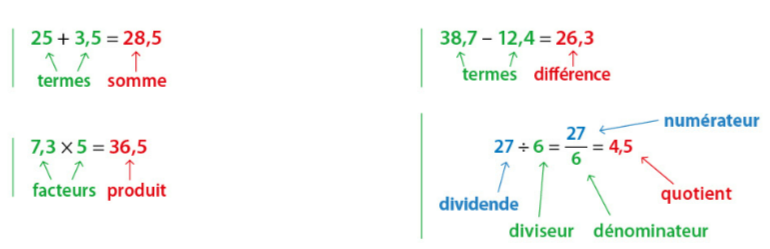
\includegraphics[width=1\linewidth]{../../assets/images/6e/seq_01/vocabualire_operations}
\end{center}
\end{examplebox}

\begin{definitionbox}
La nature d'une expression comportant plusieurs opérations est déterminée par l'opération effectuée en dernier.
\end{definitionbox}

\begin{examplebox}
Dans l'expression $2 + 3 \times 5$, c'est \trous{5cm} qu'on effectue en dernier, car la \trous{5cm} est prioritaire. Cette expression est donc une \trous{5cm}. C'est \trous{5cm} de $2$ et du \trous{5cm} de $3$ par $5$.
\end{examplebox}

\section{Exercices d'application}
\begin{exercisebox}
\textbf{Exercice 1 :} Calculer les expressions suivantes en détaillant les calculs.

\begin{enumerate}[label=\alph*)]
\item $A = 15 + 8 \times 3$
\item $B = 24 \div 6 + 5 \times 2$
\item $C = 10 - 3 \times 2 + 7$
\item $D = 18 \div (6 - 3) \times 4$
\end{enumerate}

\textbf{Exercice 2 :} Calculer les expressions suivantes.

\begin{enumerate}[label=\alph*)]
	\item $E = \frac{12 + 8}{5}$
	\item $F = \frac{30}{6 - 1}$
	\item $G = 5 \times (3 + 2 \times 4)$
	\item $H = [10 - (4 + 1)] \times 3$
\end{enumerate}

\textbf{Exercice 3 :} Identifier la nature de chaque expression (somme, différence, produit ou quotient).

\begin{enumerate}[label=\alph*)]
	\item $7 + 3 \times 2$
	\item $15 \div 3 + 4$
	\item $8 \times (5 - 2)$
	\item $\frac{20 + 4}{6}$
\end{enumerate}
\end{exercisebox}


 % Les nombres entiers

\cleardoublepage
\appendix
\chapter{Progression annuelle (récapitulatif)}
Cette progression correspond à la répartition établie pour l'année 2025–2026.

\begin{center}
\begin{tabular}{|l|l|}
\hline
\textbf{Période} & \textbf{Séquences}\\ \hline
Période 1 (6 semaines) & S01 -- Les nombres entiers, S02 -- Points et droites, S03 -- Fractions décimales et nombres décimaux\\ \hline
Période 2 (7 semaines) & S04 -- Distance, cercle et triangles, S05 -- Notion de proportionnalité, S06 -- Notion de probabilités, S07 -- Angles et rapporteur\\ \hline
Période 3 (6 semaines) & S08 -- Opérations avec les nombres décimaux, S09 -- La médiatrice d'un segment, S10 -- La division, S11 -- Symétrie axiale\\ \hline
Période 4 (7 semaines) & S12 -- Fraction partage et comparaison de fractions, S13 -- Unités de longueur, de masse et de contenance, S14 -- Calculer avec les angles, S15 -- Nombres en écriture fractionnaire\\ \hline
Période 5 (6 semaines) & S16 -- Proportionnalité et pourcentages, S17 -- Déterminer des probabilités et des issues, S18 -- Aires et périmètres, S19 -- Heures et durées, S20 -- Solides et volumes\\ \hline
\end{tabular}
\end{center}

\end{document}
